\documentclass[11pt]{article}

\usepackage{amsmath}
\usepackage{amssymb}
\usepackage{array}
\usepackage{booktabs}
\usepackage{bm}
\usepackage{caption}
\usepackage{geometry}
\usepackage{graphicx}
\usepackage{hyperref}
\usepackage{xcolor}

\geometry{a4paper, margin=1in}
\graphicspath{{figures/}}
\hypersetup{colorlinks=true, linkcolor=blue!50!black, citecolor=blue!50!black, urlcolor=blue!50!black}

\newcommand{\stream}{STREAM}
\newcommand{\cfm}{CFM}
\newcommand{\uce}{UCE}
\newcommand{\ag}{AlphaGenome}
\newcommand{\cre}{cCRE}

\title{STREAM: sequence-conditioned flow matching for developmental single-cell dynamics}
\author{}
\date{}

\begin{document}

\maketitle

\begin{abstract}
\stream{} learns continuous developmental vector fields from time-resolved
single-cell atlases while conditioning each gene's predicted velocity on linked
regulatory DNA sequence. The model combines multi-timepoint conditional flow
matching, minibatch optimal transport between neighboring stages, gene-linked
candidate cis-regulatory elements, \ag{} sequence embeddings, and optional
Universal Cell Embedding state representations. The predicted velocity and loss
are always expression-valued, so \uce{} changes the representation used to
condition the vector field rather than moving the dynamics into an embedding
space. In mouse development, expanding the modeled panel from the original
1,984 genes to 10,000 genes improved held-out timepoint prediction, and the best
model was 10k-gene \uce{} cross-attention \stream{} with full-panel MSE 20.28
and MAE 1.594. In zebrafish ZSCAPE transfer, the learned models showed a
transfer signal, with relative-time fine-tuning outperforming zero-shot and
zebrafish-only learned models, but cross-species alignment remains an open
limitation.
\end{abstract}

\section{Introduction}

Time-resolved single-cell atlases observe development as a sequence of
population snapshots. A useful dynamical model should turn those snapshots into
a continuous vector field that predicts how cell states move between stages,
while remaining comparable across genes, timepoints, and species. Conditional
flow matching provides a simulation-free way to fit such vector fields by
regressing target velocities along simple paths between empirical
distributions~\cite{lipman2023flow,tong2023minibatchot}. For developmental
data, the natural paths are between neighboring timepoints.

\stream{} extends this setup by conditioning each gene's velocity on local
regulatory sequence. For every selected gene, nearby candidate cis-regulatory
elements are embedded with \ag{}~\cite{avsec2026alphagenome}, packed as a short
regulatory token sequence, and processed by a shared gene-level transformer.
The global cell state conditions these regulatory tokens through either FiLM or
cross-attention. The readout from the promoter token is a scalar velocity for
that gene. Evaluating the shared module across all selected genes gives an
expression-space vector field.

This paper reports the current implementation and benchmarks. The main
questions are whether modeling more genes helps held-out timepoint prediction,
whether \uce{} improves the conditioning state, and whether a mouse-trained
\stream{} vector field can generalize to zebrafish after replacing gene tokens
and regulatory sequence inputs.

\section{Results}

\subsection{STREAM predicts expression-space gene velocities from cell state and regulatory sequence}

\stream{} uses two inputs at each CFM interpolation point: a cell-state vector
and a fixed set of regulatory tokens for each gene. The cell-state vector is
either expression on the selected gene panel or a frozen 1,280-dimensional
\uce{} embedding. The output is always a $G$-dimensional expression velocity,
where $G$ is the number of modeled genes (Figure~\ref{fig:model}). Thus the
dynamics, target velocity, and loss are defined in expression space even when
\uce{} is used for conditioning.

\begin{figure}[t]
\centering
\setlength{\fboxsep}{8pt}
\fbox{\begin{minipage}{0.92\linewidth}
\centering
\begin{tabular}{>{\centering\arraybackslash}p{0.17\linewidth}
                >{\centering\arraybackslash}p{0.20\linewidth}
                >{\centering\arraybackslash}p{0.22\linewidth}
                >{\centering\arraybackslash}p{0.18\linewidth}}
\textbf{expression endpoints} & \textbf{minibatch OT pair} & \textbf{interpolated state} & \textbf{expression velocity} \\
$x_k,\ x_{k+1}$ & $(x_k,x_{k+1})$ & $x_\tau$ or $u_\tau$ & $(x_{k+1}-x_k)/\Delta t$ \\
\end{tabular}

\vspace{1em}
\begin{tabular}{>{\centering\arraybackslash}p{0.22\linewidth}
                >{\centering\arraybackslash}p{0.22\linewidth}
                >{\centering\arraybackslash}p{0.22\linewidth}
                >{\centering\arraybackslash}p{0.18\linewidth}}
\textbf{linked cCREs} & \textbf{\ag{} embeddings} & \textbf{shared CRE transformer} & \textbf{promoter readout} \\
$\mathcal{C}_g$ within 100 kb & sequence token vectors & FiLM or cross-attention by state & $\hat v_g$ \\
\end{tabular}

\vspace{1em}
\textbf{Key point:} \uce{} changes the state representation supplied to the
network; \stream{} still predicts one expression velocity per gene.
\end{minipage}}
\caption{\textbf{\stream{} model structure.} Adjacent timepoints are paired by
minibatch optimal transport. The model observes an interpolated cell state and
gene-specific regulatory tokens, then predicts an expression-space velocity for
each gene.}
\label{fig:model}
\end{figure}

\subsection{Mouse held-out stages test temporal interpolation across a large developmental atlas}

The mouse benchmark uses the public single-cell transcriptional time-lapse of
mouse prenatal development~\cite{qiu2023timelapse}, represented locally as
11,441,407 cells over 24,552 genes and 43 stages from E8.5 to P0. We held out
E9.5 and E10.5 as whole timepoints. Training used only adjacent intervals whose
two endpoints were observed training stages; evaluation used intervals touching
the held-out stages. The atlas spans major developmental trajectories, and
learned vector fields can be visualized as velocity streams on the shared UMAP
(Figure~\ref{fig:mouse_atlas_velocity}).

\begin{figure}[t]
\centering
\begin{minipage}{0.44\linewidth}
\centering
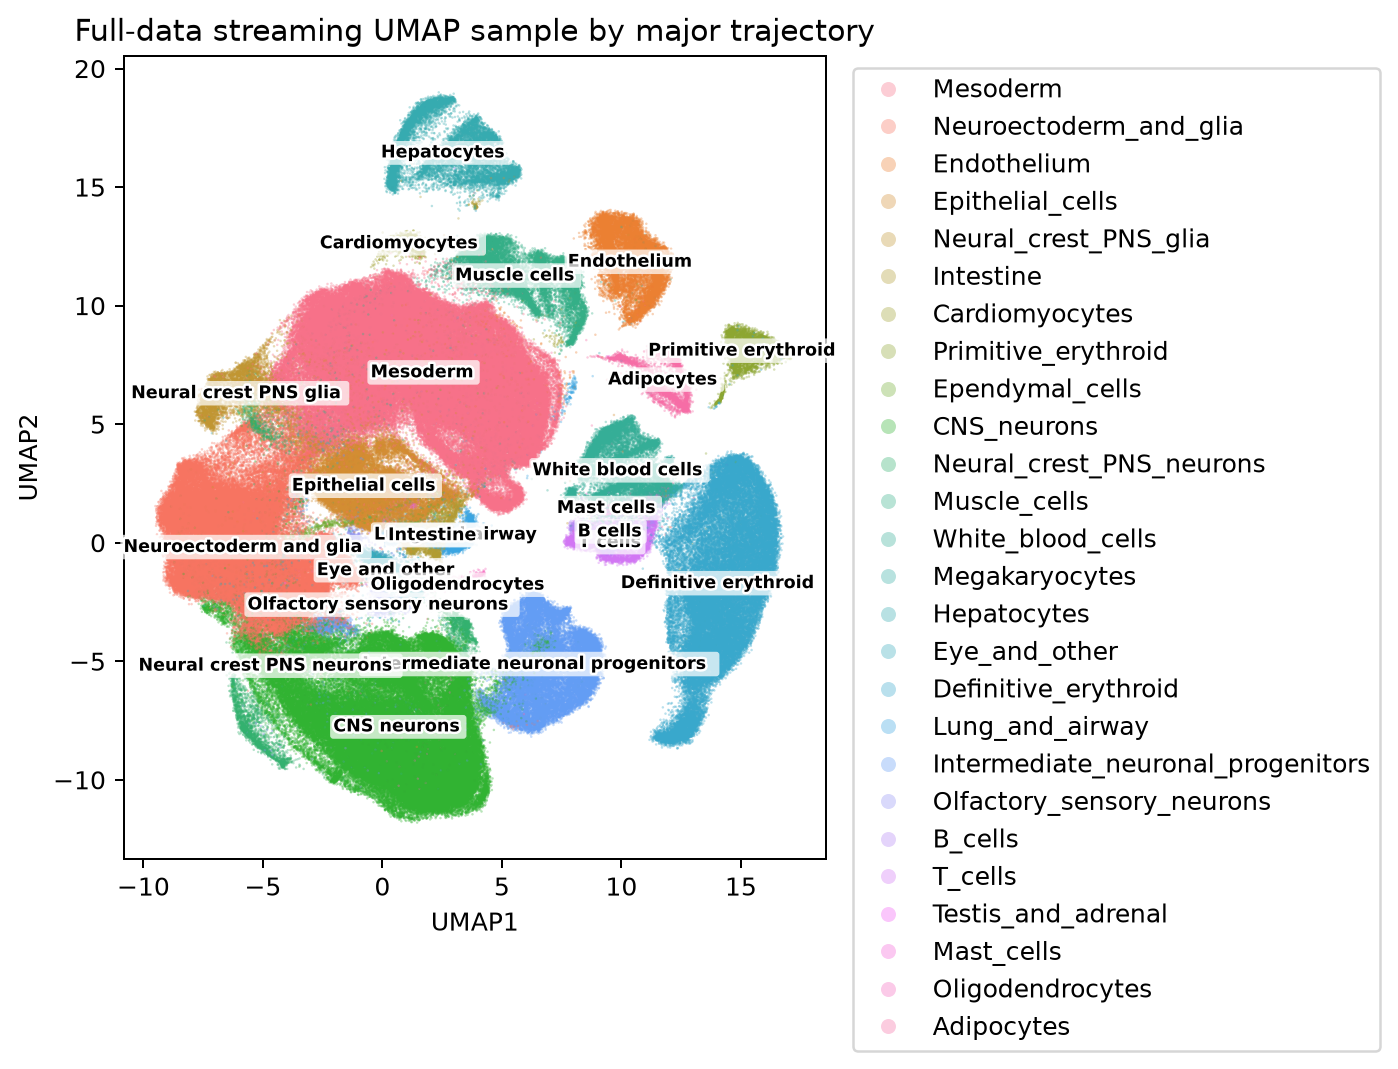
\includegraphics[width=\linewidth]{mouse_atlas_umap_major_trajectory.png}
\caption*{\textbf{A.} Mouse atlas by major trajectory.}
\end{minipage}
\hfill
\begin{minipage}{0.53\linewidth}
\centering
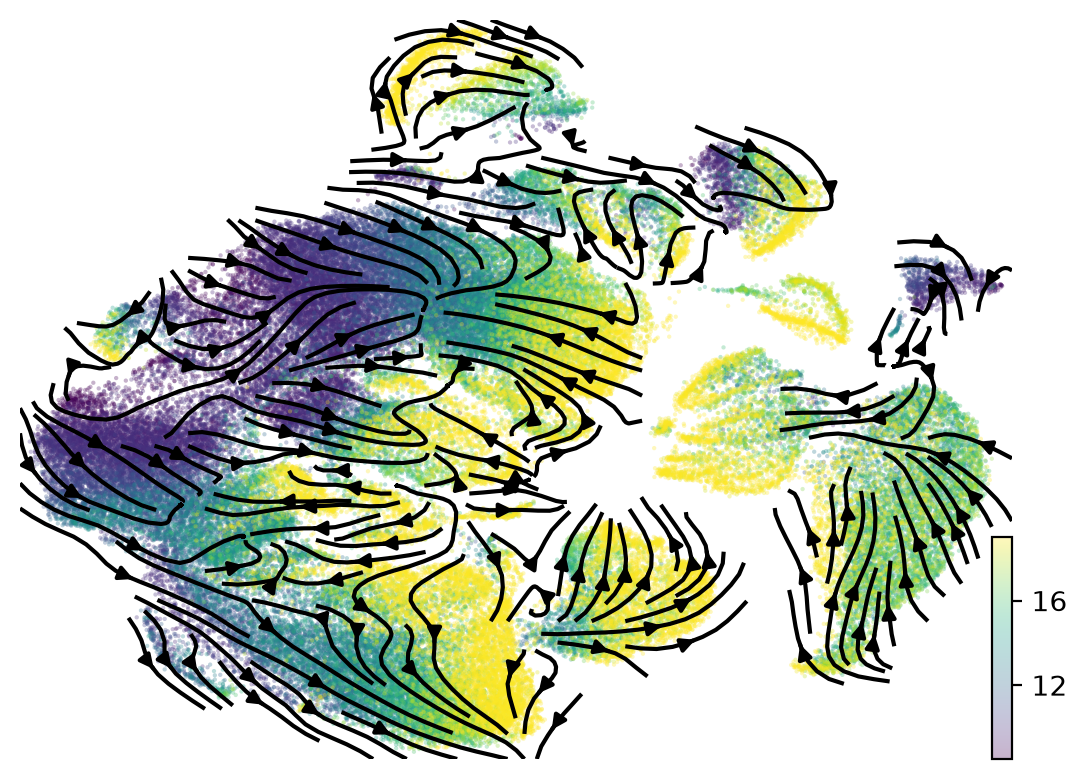
\includegraphics[width=0.32\linewidth]{velocity_embedding_stream_standard_cfm.png}
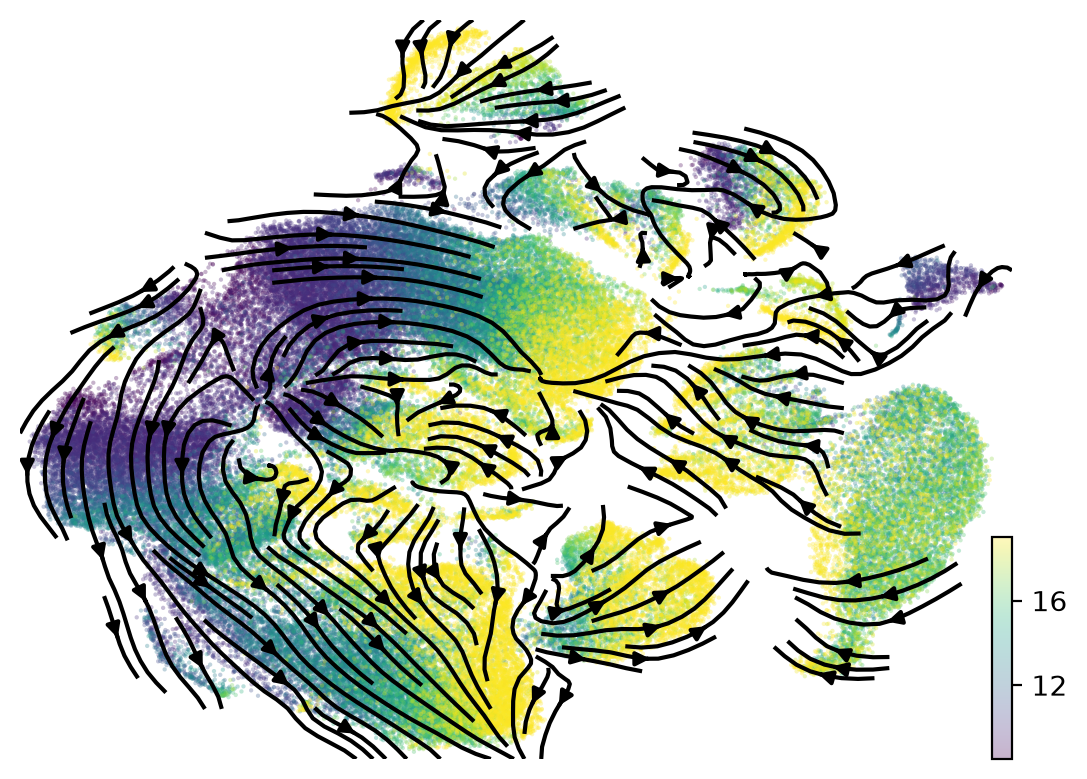
\includegraphics[width=0.32\linewidth]{velocity_embedding_stream_film.png}
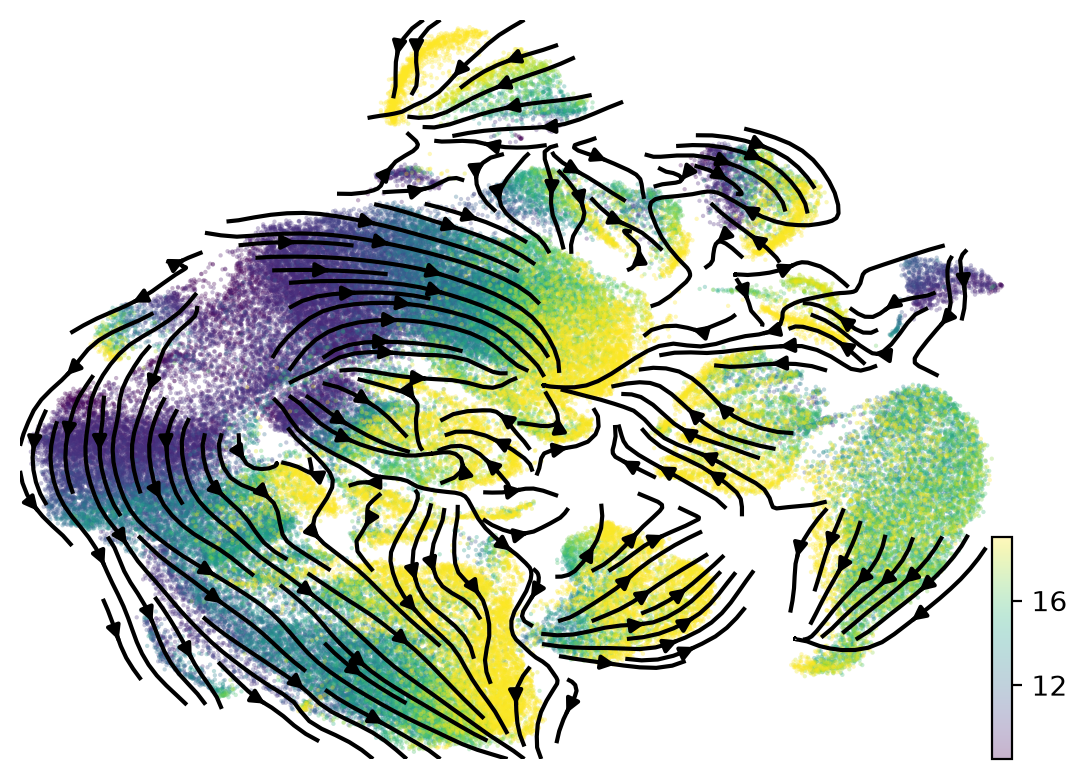
\includegraphics[width=0.32\linewidth]{velocity_embedding_stream_cross_attention.png}
\caption*{\textbf{B.} Velocity streams for CFM, FiLM STREAM, and cross-attention STREAM.}
\end{minipage}
\caption{\textbf{Mouse developmental data and learned velocity fields.}
STREAM is trained and evaluated on held-out timepoint prediction, while
velocity streams provide qualitative checks on the direction field over the
atlas manifold.}
\label{fig:mouse_atlas_velocity}
\end{figure}

\subsection{Modeling 10k genes improves mouse held-out timepoint prediction}

The original STREAM runs used a 1,984-gene panel. We reran the benchmark with
5,000 and 10,000 protein-coding highly variable genes and evaluated each model
on both its full modeled panel and the original 1,984-gene panel. Full-panel
losses decreased when moving from 5k to 10k genes for all model families
(Figure~\ref{fig:mouse_results}A). On the 10k full panel, cross-attention
\stream{} slightly improved over expression-only CFM by MSE (20.86 versus
21.16), and adding \uce{} lowered cross-attention \stream{} further to 20.28
MSE and 1.594 MAE.
Table~\ref{tab:mouse_best} summarizes the strongest 10k mouse configurations.

The fair legacy-panel comparison asks whether a larger model helps on the same
1,984 genes used by the original run. The 10k cross-attention model improved
legacy-panel MSE from 84.79 to 80.54, and 10k \uce{} cross-attention improved
it to 78.75 (Figure~\ref{fig:mouse_results}B). The 5k models did not improve
the legacy-panel metric, suggesting that the benefit is not monotonic with
panel size and appears at the 10k scale in the current setup.

\begin{figure}[t]
\centering
\begin{minipage}{0.49\linewidth}
\centering
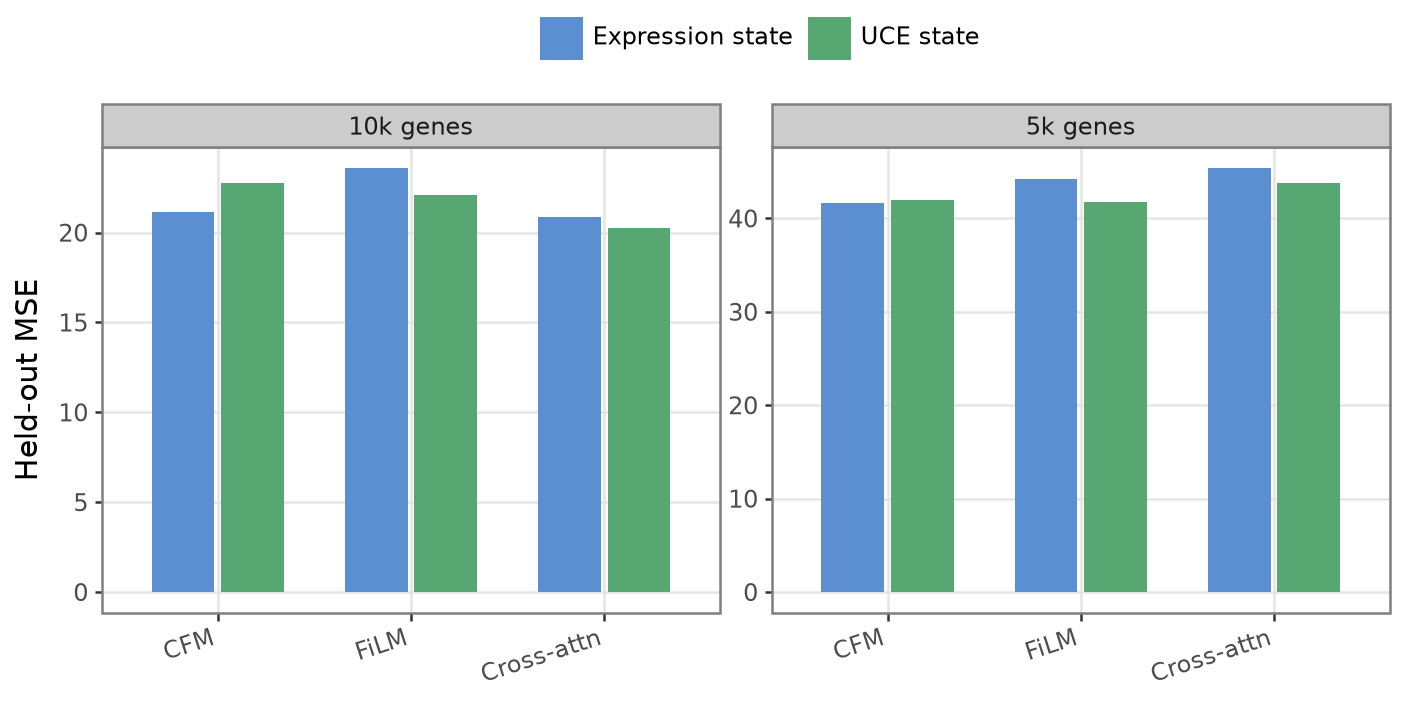
\includegraphics[width=\linewidth]{mouse_full_panel_heldout.png}
\caption*{\textbf{A.} Full modeled panel.}
\end{minipage}
\hfill
\begin{minipage}{0.49\linewidth}
\centering
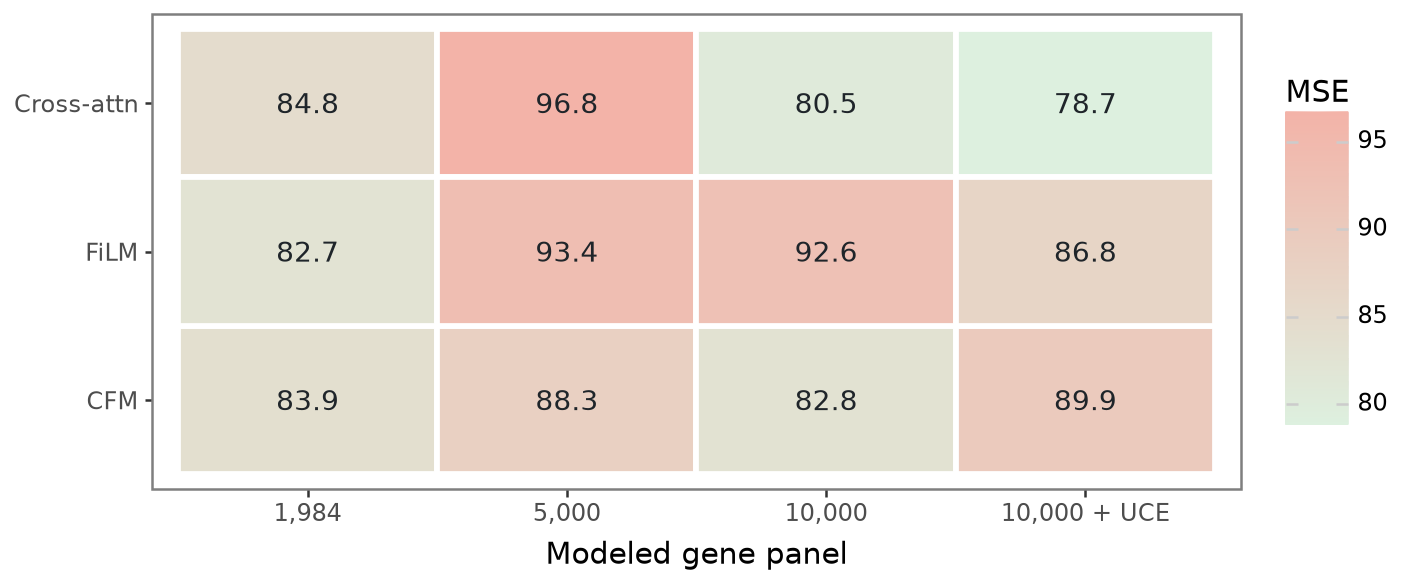
\includegraphics[width=\linewidth]{mouse_legacy_panel_heldout.png}
\caption*{\textbf{B.} Original 1,984-gene panel.}
\end{minipage}
\caption{\textbf{Mouse held-out timepoint prediction improves at 10k genes.}
Bars and heatmap entries report mean held-out MSE across cached OT evaluation
batches. Lower is better.}
\label{fig:mouse_results}
\end{figure}

\begin{table}[t]
\centering
\caption{\textbf{Best 10k mouse full-panel results.} Held-out metrics are
averaged across intervals touching E9.5 or E10.5.}
\label{tab:mouse_best}
\begin{tabular}{lrr}
\toprule
Model & MSE & MAE \\
\midrule
10k \uce{} cross-attention \stream{} & 20.28 & 1.594 \\
10k expression cross-attention \stream{} & 20.86 & 1.742 \\
10k expression CFM & 21.16 & 1.602 \\
10k \uce{} FiLM \stream{} & 22.09 & 1.629 \\
10k expression FiLM \stream{} & 23.60 & 1.669 \\
\bottomrule
\end{tabular}
\end{table}

\subsection{Zebrafish transfer shows regime-dependent learned generalization}

We next tested cross-species transfer on ZSCAPE, the zebrafish single-cell
atlas of perturbed embryos~\cite{saunders2023zscape}. The active target data
retain all 28C control cells with labels beginning \texttt{ctrl-}, giving
1,232,014 control cells before excluding cells without a modeled stage label.
Modeled stages span 18--96 hpf. We held out 36 and 72 hpf and scored intervals
touching those stages.

The transfer benchmark used the best mouse architecture: 10k-gene, \uce{}
cross-attention \stream{}. We compared a frozen mouse checkpoint applied
zero-shot to zebrafish, the same checkpoint fine-tuned on zebrafish, and a
zebrafish-only model. Cross-species scoring used expression displacement
MAE/MSE, $\lvert (f_\theta-\hat f)\Delta t \rvert$, so physical-day and
relative-time coordinates can be compared on the same expression scale.

Relative-time fine-tuning was the strongest learned zebrafish model
(displacement MAE 0.131), outperforming zero-shot (0.184) and zebrafish-only
training (0.157). Under physical-day timing, the frozen mouse checkpoint had
the lowest learned-model displacement MAE (0.175), followed by fine-tuning
(0.210) and zebrafish-only training (0.297) (Figure~\ref{fig:zfish_results};
Table~\ref{tab:zfish_results}). These results indicate a transfer signal, but
also show that cross-species alignment is sensitive to the time coordinate and
training regime.

\begin{figure}[t]
\centering
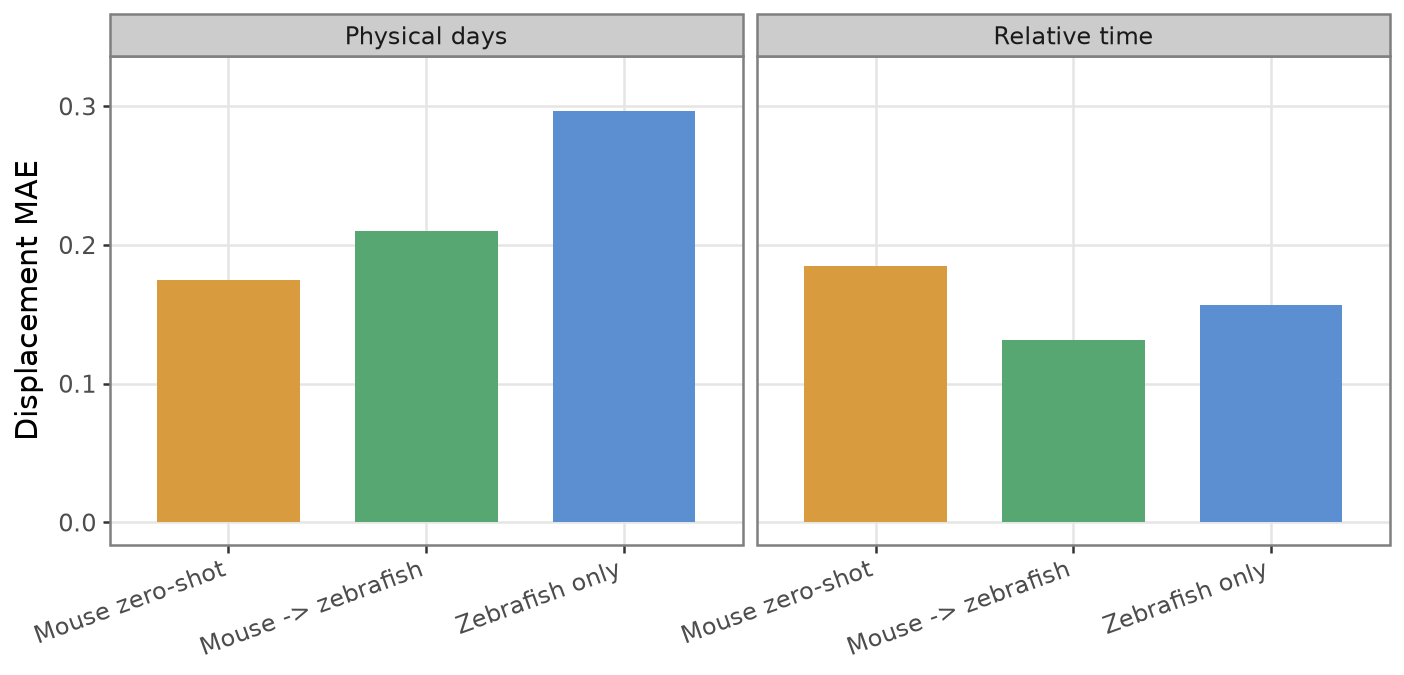
\includegraphics[width=0.86\linewidth]{zebrafish_transfer_learned.png}
\caption{\textbf{Zebrafish learned transfer results.} The plot compares only
learned models: mouse zero-shot, mouse-initialized fine-tuning, and
zebrafish-only training. Lower displacement MAE is better.}
\label{fig:zfish_results}
\end{figure}

\begin{table}[t]
\centering
\caption{\textbf{Zebrafish cross-species learned-model evaluation.} Held-out
stages are 36 and 72 hpf.}
\label{tab:zfish_results}
\begin{tabular}{llrr}
\toprule
Time coordinate & Training regime & Displacement MAE & Displacement MSE \\
\midrule
Physical days & Mouse zero-shot & 0.175 & 3.337 \\
Physical days & Mouse $\rightarrow$ zebrafish & 0.210 & 3.351 \\
Physical days & Zebrafish only & 0.297 & 3.414 \\
Relative time & Mouse zero-shot & 0.184 & 3.348 \\
Relative time & Mouse $\rightarrow$ zebrafish & 0.131 & 3.325 \\
Relative time & Zebrafish only & 0.157 & 3.331 \\
\bottomrule
\end{tabular}
\end{table}

\section{Methods}

\subsection{Data sources and regulatory annotations}

Table~\ref{tab:data_sources} summarizes the expression atlases, gene models,
genome references, and cCRE annotations used by the active analyses.

\begin{table}[t]
\centering
\caption{\textbf{Data sources used by STREAM.} Counts describe the active
analysis artifacts after project preprocessing.}
\label{tab:data_sources}
\begin{tabular}{p{0.16\linewidth}p{0.29\linewidth}p{0.25\linewidth}p{0.21\linewidth}}
\toprule
Species & Single-cell data & Gene annotation and genome & cCRE source \\
\midrule
Mouse &
JAX/Shendure mouse prenatal single-cell transcriptional time-lapse;
11,441,407 cells, 24,552 genes, 43 stages from E8.5 to P0 &
Ensembl GRCm38.95 gene models; mm10/GRCm38 genome sequence &
ENCODE/SCREEN mouse cCRE registry in mm10; 926,843 cCRE rows \\
\addlinespace
Zebrafish &
ZSCAPE 28C control embryos; 1,232,014 control cells retained before
stage filtering; modeled stages from 18 to 96 hpf &
Ensembl Danio rerio GRCz11 release 113 gene models and genome sequence &
ZEPA developmental cCRE supplement converted to GRCz11 BED; 959,040
primary cCRE rows \\
\bottomrule
\end{tabular}
\end{table}

Mouse cCREs were taken from the ENCODE/SCREEN Registry of candidate
cis-regulatory elements~\cite{encode2025ccre,screen}. Zebrafish cCREs were
taken from the ZEPA developmental chromatin accessibility supplement
(``cCREs in ZEPA and dynamic cCREs during zebrafish development'') and
converted from workbook coordinates to BED format~\cite{zepa2024,figsharezepa}.
The dynamic zebrafish workbook did not expose readable coordinate sheets in the
current conversion, so the final active BED is the primary ZEPA cCRE catalog.

For each species, protein-coding genes were selected by streaming highly
variable gene ranking and then matched to the species GTF. Mouse experiments
used the original 1,984-gene panel and rerun panels of 5,000 and 10,000 genes.
Zebrafish transfer used 10,000 genes. cCREs were linked to a gene when their
midpoint was within 100 kb of the gene transcription start site. Positive-strand
TSS coordinates used the gene start; negative-strand coordinates used the gene
end. The closest cCRE within 1 kb of the TSS was marked as the promoter token.
If no such cCRE existed, a 512 bp synthetic promoter window centered on the TSS
was inserted. Up to 32 CRE/promoter tokens were packed per gene. The 10k mouse
panel produced 317,752 linked CRE/promoter tokens; the 10k zebrafish panel
produced 318,223.

\subsection{AlphaGenome sequence embeddings}

Each real or synthetic CRE window was embedded once with the local PyTorch
\ag{} implementation. The model used 131,072 bp sequence windows and pooled the
128 bp trunk features to a 3,072-dimensional token vector. Training consumes
cached token tensors and does not call \ag{} online. The published \ag{} model
is calibrated for human and mouse organism conditioning. Zebrafish GRCz11
sequence windows therefore used the mouse organism index, which should be
treated as an out-of-distribution assumption for cross-species transfer.

\subsection{Multi-timepoint conditional flow matching}

Let $x \in \mathbb{R}^{G}$ be expression over the selected gene panel and let
$p_k(x)$ be the empirical distribution at observed timepoint $t_k$. Training is
defined over adjacent intervals $(t_k,t_{k+1})$. For a sampled pair
$(x_k,x_{k+1})$ and $\tau \sim \mathcal{U}(0,1)$,
\begin{align}
x_\tau &= (1-\tau)x_k + \tau x_{k+1}, \\
\hat v &= \frac{x_{k+1}-x_k}{t_{k+1}-t_k}.
\end{align}
The model is trained by minimizing
\begin{equation}
\mathcal{L}(\theta)=
\sum_{k}
\mathbb{E}_{\tau,(x_k,x_{k+1})}
\left[
\left\| f_\theta(s_\tau,\{\mathbf{Z}_g\}_{g=1}^{G})-\hat v \right\|_2^2
\right],
\end{equation}
where $s_\tau=x_\tau$ for expression-state runs and $s_\tau=u_\tau$ for
\uce{}-state runs. Training pairs are sampled from an entropic minibatch
optimal transport plan between cells at the two interval endpoints. The OT cost
is computed in expression space on the selected gene panel.

\subsection{UCE-state conditioning}

For \uce{} runs, a frozen 33-layer \uce{} encoder maps each endpoint cell to
$E(x)\in\mathbb{R}^{1280}$~\cite{rosen2026uce}. The same OT pair and
interpolation time are used in both spaces:
\begin{equation}
u_\tau=(1-\tau)E(x_k)+\tau E(x_{k+1}).
\end{equation}
The network input state is $u_\tau$, but the target $\hat v$, prediction, and
loss are expression-valued. Therefore \uce{} is a conditioning representation,
not the dynamical state space.

\subsection{STREAM architecture and baselines}

For gene $g$, the model receives token embeddings
$\mathbf{Z}_g=\{z_{gm}\}_{m=1}^{M}$, signed TSS-relative distances, promoter
indicators, and padding masks. The promoter token is always placed first. Token
features are projected to model width 256, augmented with signed-distance and
promoter embeddings, and processed by a shared 4-layer transformer with 8
attention heads, RoPE positional encoding, and dropout 0.1. We evaluated two
state-conditioning mechanisms:

\begin{itemize}
\item FiLM: a state MLP produces layer-specific feature-wise scale and shift
vectors applied to regulatory token states.
\item Cross-attention: a state MLP produces 8 context tokens per layer, and
regulatory tokens attend to these context tokens after CRE self-attention.
\end{itemize}

The scalar velocity for gene $g$ is read from the final promoter-token state.
Applying the same gene-level module across all genes forms
$f_\theta(s_\tau,\{\mathbf{Z}_g\}_{g=1}^{G})\in\mathbb{R}^{G}$. The
expression-only CFM baseline uses the same selected genes, same OT sampler,
same interpolation path, and same loss, but replaces sequence-conditioned gene
modules with an MLP from cell state to expression velocity.

\subsection{Held-out timepoint evaluation}

Mouse models held out E9.5 and E10.5. Zebrafish models held out 36 and 72 hpf.
All intervals touching a held-out endpoint were excluded from training and
used for evaluation. Evaluation reuses cached endpoint batches and seeded OT
sampling. Mouse metrics report velocity MSE and MAE. Zebrafish transfer reports
expression displacement MSE and MAE, computed after multiplying the velocity
error by the interval duration; this makes physical-day and relative-time
coordinates comparable on expression displacement.

\section{Discussion}

The current results support three working conclusions. First, larger gene
panels are useful at 10k genes: the improvement is visible on each model's full
output panel and persists on the original 1,984-gene panel for cross-attention
\stream{}. Second, \uce{} helps the sequence-conditioned models more than the
expression-only CFM baseline, consistent with the idea that a cross-species cell
state representation is most useful when each gene can query state context
through its own regulatory tokens. Third, cross-species generalization is not
solved by swapping annotations alone. Mouse-to-zebrafish transfer depends on
time scaling and on whether the model is fine-tuned in the target species.

The main limitations are the simple TSS-window CRE linking rule, the lack of
zebrafish-specific \ag{} calibration, and the short-interval held-out endpoint
metric. Future work should test cell-type-aware regulatory links, sequence
embeddings trained or calibrated for zebrafish, explicit time conditioning, and
rollout-based evaluation in addition to endpoint displacement.

\begin{thebibliography}{99}

\bibitem{lipman2023flow}
Lipman, Y., Chen, R. T. Q., Ben-Hamu, H., Nickel, M. \& Le, M.
Flow Matching for Generative Modeling.
\textit{International Conference on Learning Representations} (2023).
\url{https://arxiv.org/abs/2210.02747}

\bibitem{tong2023minibatchot}
Tong, A., Fatras, K., Malkin, N., Huguet, G., Zhang, Y.,
Rector-Brooks, J., Wolf, G. \& Bengio, Y.
Improving and generalizing flow-based generative models with minibatch optimal transport.
\textit{Transactions on Machine Learning Research} (2024).
\url{https://arxiv.org/abs/2302.00482}

\bibitem{qiu2023timelapse}
Qiu, C. et al.
A single-cell transcriptional timelapse of mouse embryonic development, from gastrula to pup.
\textit{bioRxiv} (2023).
\url{https://doi.org/10.1101/2023.04.05.535726}

\bibitem{saunders2023zscape}
Saunders, L. M. et al.
Embryo-scale reverse genetics at single-cell resolution.
\textit{Nature} \textbf{623}, 782--791 (2023).
\url{https://doi.org/10.1038/s41586-023-06720-2}

\bibitem{rosen2026uce}
Rosen, Y. et al.
Universal cell embedding provides a foundation model for cell biology.
\textit{Nature} (2026).
\url{https://doi.org/10.1038/s41586-026-10689-z}

\bibitem{avsec2026alphagenome}
Avsec, Z. et al.
Advancing regulatory variant effect prediction with AlphaGenome.
\textit{Nature} \textbf{649}, 1206--1218 (2026).
\url{https://doi.org/10.1038/s41586-025-10014-0}

\bibitem{encode2025ccre}
ENCODE Project Consortium.
An expanded registry of candidate cis-regulatory elements.
\textit{Nature} (2025).
\url{https://pmc.ncbi.nlm.nih.gov/articles/PMC11703161/}

\bibitem{screen}
ENCODE SCREEN.
Search candidate cis-regulatory elements by ENCODE.
\url{https://screen.encodeproject.org/}

\bibitem{zepa2024}
Mapping the chromatin accessibility landscape of zebrafish embryogenesis at single-cell resolution by SPATAC-seq.
\textit{PubMed record} (2024).
\url{https://pubmed.ncbi.nlm.nih.gov/38977847/}

\bibitem{figsharezepa}
Supplemental data for ZEPA.
\textit{Figshare} (2024).
\url{https://figshare.com/articles/dataset/supplemental_data_for_ZEPA/25465477}

\end{thebibliography}

\end{document}
